In this chapter we will describe the architecture of the entire system by first showing the overall structure followed by a short description of the individual components. 
The platform is able to accomodate the ability for lecturers to create a syllabus that includes problemsets, exercises and test cases for the exercises. Additionally, the platform has the ability for students to do the exercises that the lecturer has provided. 
The platform is a web application, consisting of a user-interface, business logic to handle requests, authentication and compilation of the code as well as a database to persist relevant data.
The overall architecture for the system can be seen in figure \ref{fig:Architecture}.

\begin{figure}[H]
	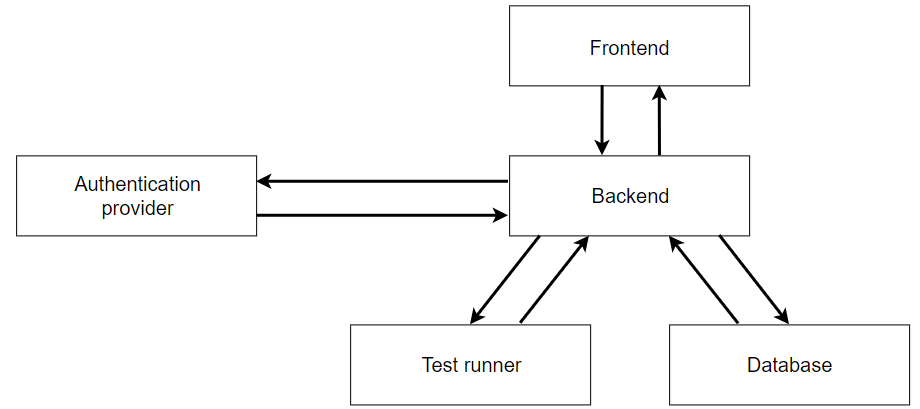
\includegraphics[scale=0.6]{Architecture.PNG}
	\centering
	\caption{The architecture for our web application}
	\label{fig:Architecture}
\end{figure}

The architecture for the system is based on a client-server structure. Additionally, we have added an API running a separate server instance to handle code execution and test, called \textit{Test runner}. As each component is introduced, in the following sections, we will elaborate on the choices made for each component, in relation to this structure.

\section{Frontend}
The frontend is the user facing component of our web application. The frontend is designed such that its user-interface and functionality is dependent on the role of the user. 
For example if a student has signed in, the student is able to see and complete exercises. In turn if a lecturer signs in, they will have access to more functionality such as creating a syllabus or exercise.

Regardless of the roles of the user the frontend has the ability to persist data and execute code through communication with the backend system.

\section{Back-end system}
The backend system has several responsibilities including routing, data retrieval and updates, execution of code tests and communication with an authentication provider. The backend provides all the functionality that is essential to our web application. It operates as a traditional server in a client-server architechture. 

\subsection*{Authentication provider}


\section{Database}
In order persist data, the backend retrieves and updates data in the database component depicted in figure \ref{fig:Architecture}. This is done through create, read, update and delete operations. 
The backend then queries the database and returns the relevant data. 

The database component is implemented as a Postgres database. The entities and their relationships contained within the database is shown in figure \ref{fig:Database}. In the figure each box represents an entity-set and attributes for the entities. A diamond represent a relationship between two or more entity-sets.

A dotted line connecting an entity-set to a relationship represent a partial participation of the connected entities and the other participants in the relationship. This means that an entity can exist in the database without participating in the relationship.
A full line connecting an entity-set to a relationship represents total participation of the entity-set symbolising that an entity must participate in the relationship. 
This means that an entity cannot exist in the database without participating in the relationship.
The numbers and letters at the beginning of each relationship line represents the cardinality. A \textit{number} between a relationship and an entity-set represents the number of times an entity can participate in the relationship. Similarily, an \textit{N} represents that entities can participate $0$ or more times.

\begin{figure}[H]
	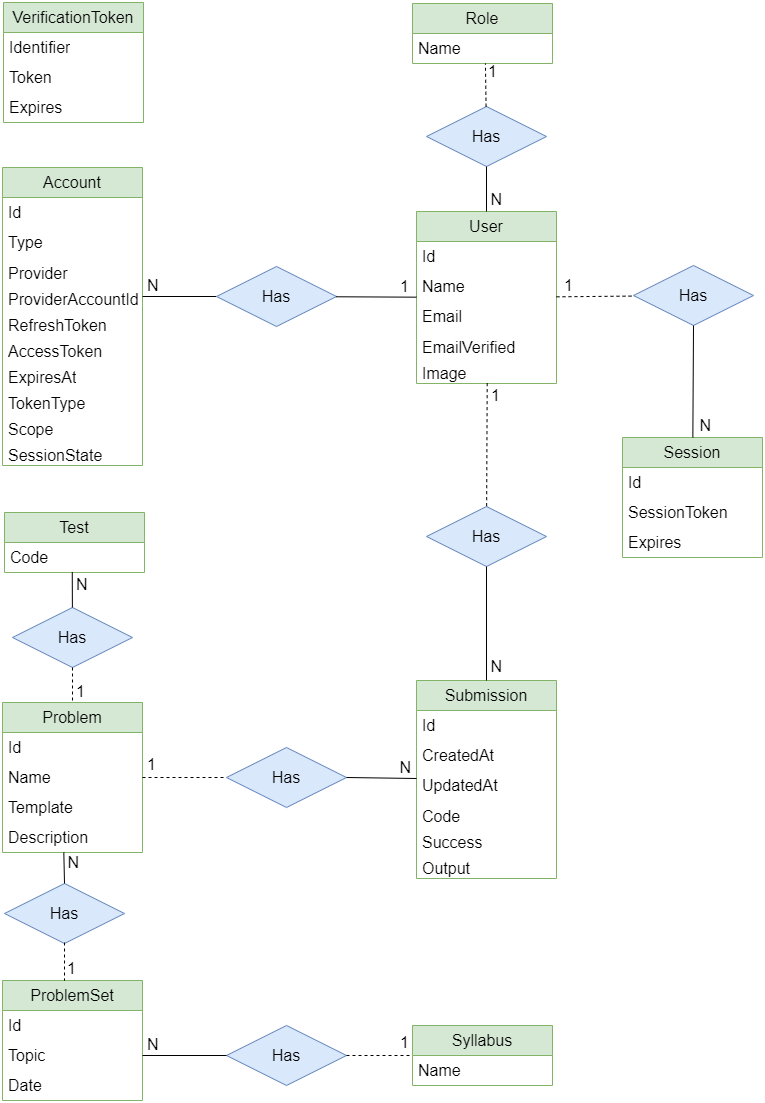
\includegraphics[scale=0.4]{Database.png}
	\centering
	\caption{Entity relationship diagram of the database}
	\label{fig:Database}
\end{figure}

The structure of database can be explained through the two types of users of the system. The lecturer and the student.
In order to support different roles in the system, we have created the entites \textit{Role} and \textit{User}. The \textit{Role} entity has one attribute called \textbf{Name}. This corresponds to the name of the role. The \textit{User} entity has the attributes \textbf{Id}, which is a unique identifier, \textbf{Name}, \textbf{Email}, \textbf{EmailVerifed} which is when the email was verified and an \textbf{Image} attribute which contains an image of the user (Is a string type in DB - pl0x explain). The \textit{User} entity has a many-to-one relationship with the entity \textit{Role}, which means that users can only have one role.

To support a lecturer in creating a syllabus for a semester course we have created the entities \textit{Syllabus}, \textit{Problemset}, \textit{Problem} and \textit{test}. For each entity, a set of attributes and relationships have been added to contain the relevant data.
For the \textit{Problem} entity we have added an \textbf{Id} attribute as a unique identifier, a \textbf{Name} attribute, a \textbf{Template} attribute, which contains code that will be automatically included in the editor when starting a problem. This ensures that the functions that required for the tests are included, as described in section Hspec (Need proper ref - May not be hspec). The final attribute is the \textbf{Description}, which contains the description of the exercise.

The \textit{Test} entity has the attribute \textbf{Code}. This contains the test code that the lecturer has written for a problem. A \textit{Problem} and a \textit{Test} are in a one-to-many relationship with each other, where a \textit{Problem} has many \textit{tests}. This allows a lecturer to define multiple tests for a problem.

The \textit{Problemset} entity corresponds to a course exercise session. It has the attribute \textbf{Id}, which a unique identifier, the attribute \textbf{Topic} which is the topic covered in the session, and lastly a \textbf{Date} which corresponds the when the session occurs. The relationship between the \textit{Problemset} entity and the \textit{Problem} entity is one-to-many, since a problemset has multiple problems. This allows the lecturer to create a set of problems for a course exercise session.

The \textit{Syllabus} entity corresponds to an entire syllabus for a course. The entity only has a \textbf{Name} attribute, which is the name of the course. The \textit{Syllabus} entity has a one-to-many relationship with the \textit{Problemset} entity. This allows the lecturer to create multiple problem sets for a course.

To support a student in submitting solutions to exercises we have created the entity \textit{Submission}. This entity contains the attributes \textbf{Id}, which is a unique identifier, \textbf{CreatedAt} which contains the time for when the submission was first added, \textbf{UpdatedAt} which contains the time when the submission was last updated. It also contains the attributes \textbf{Code}, which contains the code submitted by the student, \textbf{Success} which states whether the submission passed the tests for the problem. Finally it has the attribute \textbf{Output}, which is the standard output from the compiler.
The \textit{Submission} entity is in a many-to-one relationship with the \textit{User} entity, because each user can have many submissions. \textit{Submission} is also in a many-to-one relationship with \textit{Problem}, as a problem can have multiple submissions.

The remaining entities \textit{Account}, \textit{Session} and \textit{VerificationToken} are entities which are required by the authentication service and are not developed by us. (Are they specific to google auth?)

\section{Test runner}
As mentioned previously the platform is able run code on back-end and verify whether this code is syntactically correct and safisfies the lecturer defined tests.
The component is structured as a layered architecture where each layer is a module and each module has a single responsibility with no global state and full encapsulation.
This means that each component can depend only on components on a lower or same level. For example if component A is on a lower level than component B, component A cannot use component B.
This makes the architecture decoupled and therefore it is easy to add, replace and modify components.

The component structure can be seen in figure \ref{fig:TestRunner}

\begin{figure}[H]
	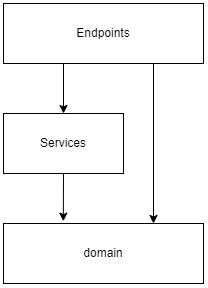
\includegraphics[scale=0.4]{TestRunner.jpg}
	\centering
	\caption{The test runner component architecture}
	\label{fig:TestRunner}
\end{figure}

\subsection{Authentication provider}


